% !TeX root = ../../Book3.tex
% 纲要标题：### 2.4 割迹与注入半径
% 纲要位置：几何学计划纲要.md，第 2183 行。
% 正文状态：初稿；尚未正式审核。

% 纲要内容开始
% 
% * 最大极小区间与割点函数
% * 指数映射的单射范围
% * 注入半径及紧流形下界
% * 球面、平坦环面和商空间模型
% 
% ---
% 
% 纲要内容结束

\section{割迹与注入半径}
\label{g3:sec:0204}

在一个法邻域内，径向测地线既唯一又最短；把它继续延长，这两个性质都可能改变。圆周上的短弧到达对径点时出现另一条等长弧，越过对径点后原来的弧就不再最短。我们先沿每个方向记录这种变化，再讨论指数映射在哪些半径内仍能给出坐标。本节除另有说明外，假设 \((M,g)\) 连通、完备、无边界，且维数 \(n\ge1\)。

\subsection{最大极小区间与割点函数}
\label{g3:subsec:0204:01}
固定 \(p\in M\)，记 \(S_pM=\{u\in \mathrm{T}_pM:|u|_g=1\}\)，并令 \(\gamma_u(t)=\exp_p(tu)\)。完备性保证它对所有实数 \(t\) 有定义。沿这条单位速测地线，长度总是参数差，端点距离却可能更小。

\begin{definition}[割时与割迹]\label{g3:def:cut-time}
	方向 \(u\in S_pM\) 的\term[geshi]{割时}[cut time]定义为
	\[
		c_p(u)=\sup\{t\ge0:d(p,\gamma_u(t))=t\}\in(0,\infty].
	\]
	若 \(c_p(u)<\infty\)，称 \(\gamma_u(c_p(u))\) 为该方向的\term[gedian]{割点}[cut point]。所有这样的点组成 \(p\) 的\term[geji]{割迹}[cut locus]，记为
	\[
		\operatorname{Cut}(p)=\{\exp_p(c_p(u)u):u\in S_pM,\ c_p(u)<\infty\}.
	\]
	\symidx{\(c_p(u)\)}
	\symidx{\(\operatorname{Cut}(p)\)}
\end{definition}

定义中的集合确实是一个区间。若 \(d(p,\gamma_u(t))=t\) 且 \(0\le s\le t\)，三角不等式给出
\[
	t=d(p,\gamma_u(t))\le d(p,\gamma_u(s))+(t-s)\le s+(t-s)=t.
\]
因此两处不等式都取等号，\(d(p,\gamma_u(s))=s\)。\cref{g3:prop:normal-radial-minimality}又保证足够小的正数 \(s\) 满足这个等式，所以 \(c_p(u)>0\)。若 \(c_p(u)\) 有限，距离的连续性使等式在端点仍成立。于是最大极小区间是 \([0,c_p(u)]\)；若割时无穷，就是 \([0,\infty)\)。在有限割时之后，每个 \(t>c_p(u)\) 都满足严格不等式 \(d(p,\gamma_u(t))<t\)。

\ProseParagraphBreak

这里的“极小”表示这段曲线在所有连接端点的曲线中长度最小。每条测地线在每个参数值附近仍有足够短的极小子段；越过割点所失去的是从原起点 \(p\) 算起的整体极小性。

\begin{proposition}\label{g3:prop:cut-time-upper-semicontinuity}
	割时函数 \(c_p:S_pM\to(0,\infty]\) 是上半连续的：若 \(u_j\to u\)，则
	\[
		\limsup_{j\to\infty}c_p(u_j)\le c_p(u).
	\]
\end{proposition}
\begin{proof}
	设 \(t<c_p(u_j)\) 对某个子列的所有项成立。沿该子列有 \(d(p,\exp_p(tu_j))=t\)；由指数映射与距离的连续性，极限给出 \(d(p,\exp_p(tu))=t\)，所以 \(t\le c_p(u)\)。若上极限大于 \(c_p(u)\)，在二者之间取这样的 \(t\) 即得矛盾。\(c_p(u)=\infty\) 时不等式自动成立。
\end{proof}

上半连续性说明：当极小线段的初方向与长度同时收敛时，极限线段仍极小。它来自端点距离等式的封闭性，不需要曲率计算。

\subsection{指数映射的单射范围}
\label{g3:subsec:0204:02}
令
\[
	\mathcal D_p=\{0\}\cup\{tu:u\in S_pM,\ 0<t<c_p(u)\}\subset \mathrm{T}_pM.
\]
这保留每条射线上严格位于割时之前的向量。以下结论首先说明它在集合意义上如何参数化割迹的补集。

\begin{proposition}[割点之前的唯一性]\label{g3:prop:precut-injectivity}
	若 \(0<t<c_p(u)\)，则 \(\gamma_u|_{[0,t]}\) 是从 \(p\) 到 \(q=\gamma_u(t)\) 的唯一单位速最短测地线。指数映射限制给出双射
	\[
		\exp_p:\mathcal D_p\longrightarrow M\setminus\operatorname{Cut}(p).
	\]
\end{proposition}
\begin{proof}
	取 \(\varepsilon>0\)，使 \(t+\varepsilon<c_p(u)\)。若另有一条从 \(p\) 到 \(q\) 的单位速最短测地线 \(\sigma:[0,t]\to M\)，将它与 \(\gamma_u|_{[t,t+\varepsilon]}\) 拼接，所得曲线长 \(t+\varepsilon\)，仍等于两端距离。由\cref{g3:lem:corner-shortening}，接点不能有角点，所以 \(\dot\sigma(t)=\dot\gamma_u(t)\)。测地线初值唯一性向后应用，得到 \(\sigma=\gamma_u|_{[0,t]}\)。

	\(\mathcal D_p\) 中的非零向量长度等于其像到 \(p\) 的距离。同一点的两个原像因而有相同长度，由刚证的唯一性又有相同方向，故限制映射单射。若其像 \(q\) 同时为某个方向的割点，沿那个方向到 \(q\) 的线段也是最短线，只能与已有线段相同；这样同一方向的同一参数既小于割时又等于割时，矛盾。

	最后取 \(q\notin\operatorname{Cut}(p)\)、\(q\ne p\)。Hopf--Rinow 定理给出一条从 \(p\) 到 \(q\) 的单位速最短测地线，写成 \(\gamma_u|_{[0,t]}\)，其中 \(t=d(p,q)\le c_p(u)\)。等号会使 \(q\) 成为割点，所以 \(t<c_p(u)\)。点 \(p\) 则由零向量表示。
\end{proof}

这个证明还给出一个实用判据：若同一点由两条不同的最短测地线到达，则它必在起点的割迹中。反向陈述并不由唯一性证明得到。割时处指数映射的微分也可能发生退化；下面把这两种可能性分开。

\begin{proposition}[有限割时处的两种可能]\label{g3:prop:cut-endpoint-alternative}
	设 \(c=c_p(u)<\infty\)，\(q=\exp_p(cu)\)。则至少发生下列一件事：
	\begin{enumerate}
		\item 从 \(p\) 到 \(q\) 存在两条不同的最短测地线；
		\item \((\mathrm d\exp_p)_{cu}\) 不可逆。
	\end{enumerate}
\end{proposition}
\begin{proof}
	假设最短测地线唯一，且该微分可逆。取 \(t_j\downarrow c\)、\(t_j>c\)，令 \(q_j=\exp_p(t_ju)\)。由 Hopf--Rinow 定理，可取 \(v_j\in \mathrm{T}_pM\)，使
	\[
		\exp_p(v_j)=q_j,\qquad |v_j|=d(p,q_j)<t_j.
	\]
	距离连续性给出 \(|v_j|\to c\)。有限维切空间中的有界序列有收敛子列，记极限为 \(v\)。则 \(|v|=c\)、\(\exp_p(v)=q\)，相应径向线长等于端点距离，故是最短线。唯一性使 \(v=cu\)。逆函数定理给出 \(cu\) 的一个邻域，\(\exp_p\) 在其中单射。子列的 \(v_j\) 与 \(t_ju\) 最终都在此邻域内，像相同，却因长度不同而不相等，矛盾。
\end{proof}

微分退化如何由沿测地线的变分场检测，将在\cref{g3:sec:0602}建立。\cref{g3:sec:0603}再把它与割时联系起来。这里的双射与上述二择结论已经足以解释以下模型中指数坐标失效的位置。

\subsection{注入半径及紧流形下界}
\label{g3:subsec:0204:03}
即使不假设完备，\cref{g3:prop:exponential-local}也保证指数映射在零向量附近是微分同胚。以整个切球作为坐标范围所能达到的最大半径，给出一个可以逐点比较的尺度。

\begin{definition}[注入半径]\label{g3:def:injectivity-radius}
	对无边界黎曼流形上的 \(p\)，定义 \(p\) 的\term[zhurubanjing]{注入半径}[injectivity radius]为
	\[
		\operatorname{inj}_g(p)=\sup\bigl\{r>0:\exp_p\text{ 在 }B_r(0)\subset \mathrm{T}_pM
		\text{ 上有定义且为到其像的微分同胚}\bigr\}.
	\]
	流形的注入半径定义为 \(\operatorname{inj}_g(M)=\inf_{p\in M}\operatorname{inj}_g(p)\)。上确界允许为无穷，整体下确界则可能为零。
	\symidx{\(\operatorname{inj}_g(p)\)}
\end{definition}

\begin{proposition}\label{g3:prop:compact-injectivity-lower-bound}
	每点的注入半径为正，且在任意紧子集上有统一正下界。特别地，紧黎曼流形的注入半径为正。若流形还完备，则对 \(0<r<\operatorname{inj}_g(p)\)，
	\[
		\exp_p(B_r(0))=B_d(p,r),\qquad
		d(p,\exp_p v)=|v|\quad(|v|<r),
	\]
	并且 \(\operatorname{inj}_g(p)\le\inf_{u\in S_pM}c_p(u)\)。
\end{proposition}
\begin{proof}
	逐点正性来自逆函数定理。\cref{g3:lem:uniform-normal-neighborhood}进一步给出：每点 \(p\) 有邻域 \(V_p\) 和常数 \(r_p>0\)，使所有 \(x\in V_p\) 的指数映射在 \(B_{r_p}(0)\subset \mathrm{T}_xM\) 上均为微分同胚。有限个 \(V_p\) 覆盖给定紧集；取对应 \(r_p\) 的最小值即可。

	现在假设完备，并取 \(r<\operatorname{inj}_g(p)\)。对 \(|v|<r\)，径向线给出 \(d(p,\exp_pv)\le|v|\)。若严格小于，取一条最短测地线，把其初向量按终点参数一缩放为 \(w\)，便有 \(|w|=d(p,\exp_pv)<|v|<r\) 且 \(\exp_pw=\exp_pv\)，与切球内的单射性矛盾。因此距离等式成立。反过来，\(d(p,q)<r\) 时最短测地线给出长度小于 \(r\) 的原像，所以像正是距离球。对每个方向与所有 \(t<r\) 应用距离等式，得到 \(c_p(u)\ge r\)；让 \(r\) 趋向注入半径即得最后的不等式。
\end{proof}

这一正下界的证明只用局部指数映射和紧性。在非紧流形上，各点都有法邻域，却未必能选同一个半径。习题中的尖缩圆柱会给出完备但整体注入半径为零的例子。一般流形上注入半径与最早割时的相等关系，连同割时函数的进一步正则性，将随第6章的指数映射微分理论完成。

\subsection{球面、平坦环面和商空间模型}
\label{g3:subsec:0204:04}
\begin{example}[圆球面的割迹]\label{g3:exm:sphere-cut-locus}
	在半径 \(a\) 的圆球面 \(S_a^n\)、\(n\ge1\) 上，\cref{g3:exm:round-sphere-exponential}给出
	\[
		\exp_p(tu)=\cos(t/a)p+a\sin(t/a)u\qquad(|u|=1).
	\]
	这些曲线全时存在，所以球面完备。对 \(q\ne p\)，取到 \(q\) 的最短测地线，长度记为 \(\ell\)。显式公式中长度超过 \(\pi a\) 的弧总能换成同一大圆上长度至多 \(\pi a\) 的弧：先减去整圈，再在长弧和短弧之间选择。因此 \(0<\ell\le\pi a\)，并且
	\[
		d(p,q)=a\arccos\frac{\langle p,q\rangle}{a^2}.
	\]
	从而 \(c_p(u)=\pi a\) 对所有方向成立，\(\operatorname{Cut}(p)=\{-p\}\)。指数映射在 \(B_{\pi a}(0)\) 上是到去掉对径点的球面的微分同胚，而任意更大的切球内都有两个向量 \(\pi a u\)、\(-\pi a u\) 映到 \(-p\)。故
	\[
		\operatorname{inj}(S_a^n)=\pi a.
	\]
	当 \(n=1\)，到对径点有两条半圆最短弧；当 \(n\ge2\)，每个单位初方向都给出一条最短半大圆。对于 \(n=1\)，指数映射在割时处仍是局部微分同胚，失效的是单射性。
\end{example}

\begin{example}[平坦环面的最近格点区域]\label{g3:exm:flat-torus-cut-locus}
	设 \(\Lambda\subset\mathbb R^n\) 为由一组基生成的格，\(T=\mathbb R^n/\Lambda\) 取 Euclid 度量诱导的商度量。商映射在足够小的球上是等距坐标图，所以测地线就是直线的投影，且 \(T\) 完备。若 \(p=[x]\)、\(q=[y]\)，每条从 \(p\) 到 \(q\) 的曲线从 \(x\) 提升后终止于某个 \(y+\lambda\)，长度不变；其长度至少为 \(|y-x+\lambda|\)。直线段达到该下界。因此
	\begin{equation}\label{g3:eq:flat-torus-distance}
		d_T([x],[y])=\min_{\lambda\in\Lambda}|y-x+\lambda|.
	\end{equation}
	最小值确实取得：任何有界 Euclid 球只含有限个格点。所用路径提升来自第一卷第5.3节的道路提升定理；这里的平移商在小球上满足其均匀覆盖条件。局部逆光滑，所以分片光滑曲线的提升也分片光滑。

	将 \(\mathrm{T}_pT\) 与 \(\mathbb R^n\) 认同，则 \(\exp_pv=[x+v]\)。定义格的最近点区域
	\[
		V=\{v\in\mathbb R^n:|v|\le|v-\lambda|\text{ 对所有 }\lambda\in\Lambda\}
		=\bigcap_{\lambda\in\Lambda\setminus\{0\}}
		\{v:2\langle v,\lambda\rangle\le|\lambda|^2\}.
	\]
	它是闭凸集。取一个有界的基本平行多面体，可知任一点到格的距离有统一上界；\(v\in V\) 时最近格点是零，故 \(|v|\) 也有统一上界，所以 \(V\) 有界。在任意有界区域内，足够长的格向量自动满足严格不等式，因而只有有限个不等式影响边界。由此，\(V\) 的内部由所有严格不等式刻画，边界点至少满足一个非零格向量对应的等式。

	径向线段到 \([x+tu]\) 最短，当且仅当 \(tu\in V\)。每条射线与 \(V\) 相交为一个闭区间，所以
	\[
		c_p(u)=\min_{\substack{\lambda\in\Lambda\\\langle u,\lambda\rangle>0}}
		\frac{|\lambda|^2}{2\langle u,\lambda\rangle},\qquad
		\operatorname{Cut}(p)=[x+\partial V].
	\]
	式中的最小值存在：\(V\) 有界使射线在有限参数退出，而该边界点处有一个起约束作用的格向量。若 \(v\in\partial V\) 且 \(|v|=|v-\lambda|\)，向量 \(v\) 与 \(v-\lambda\) 给出同一终点的两条最短线。切空间中的相邻区域因此在割迹上发生识别。

	设 \(\ell_\Lambda=\min_{\lambda\ne0}|\lambda|\)。指数映射微分处处可逆；若 \(|v|,|w|<\ell_\Lambda/2\) 且像相同，则 \(v-w\in\Lambda\)，但 \(|v-w|<\ell_\Lambda\)，故 \(v=w\)。任意大于 \(\ell_\Lambda/2\) 的切球又包含一对 \(\lambda/2,-\lambda/2\)，其中 \(|\lambda|=\ell_\Lambda\)，它们像相同。于是
	\[
		\operatorname{inj}(T)=\tfrac12\ell_\Lambda.
	\]
\end{example}

\begin{figure}[htbp]
	\centering
	% !TeX root = ../Book3.tex
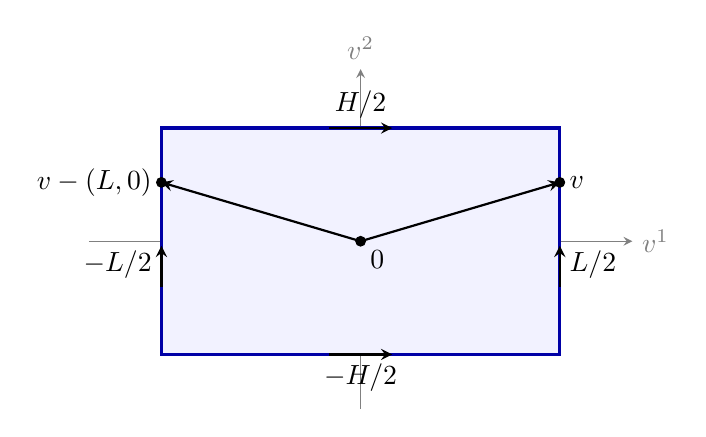
\begin{tikzpicture}[scale=1.15,>=stealth]
	\draw[->,gray] (-3.0,0)--(3.0,0) node[right] {\(v^1\)};
	\draw[->,gray] (0,-1.85)--(0,1.9) node[above] {\(v^2\)};
	\fill[blue!5] (-2.2,-1.25) rectangle (2.2,1.25);
	\draw[very thick,blue!65!black] (-2.2,-1.25) rectangle (2.2,1.25);
	\draw[thick,->] (0,0)--(2.2,0.65);
	\draw[thick,->] (0,0)--(-2.2,0.65);
	\fill (0,0) circle (1.7pt) node[below right] {\(0\)};
	\fill (2.2,0.65) circle (1.7pt) node[right] {\(v\)};
	\fill (-2.2,0.65) circle (1.7pt) node[left] {\(v-(L,0)\)};
	\node[below] at (0,-1.25) {\(-H/2\)};
	\node[above] at (0,1.25) {\(H/2\)};
	\node[below right] at (2.2,0) {\(L/2\)};
	\node[below left] at (-2.2,0) {\(-L/2\)};
	\draw[->,thick] (-0.35,1.25)--(0.35,1.25);
	\draw[->,thick] (-0.35,-1.25)--(0.35,-1.25);
	\draw[->,thick] (2.2,-0.5)--(2.2,-0.05);
	\draw[->,thick] (-2.2,-0.5)--(-2.2,-0.05);
\end{tikzpicture}

	\caption[矩形平坦环面的割迹]{矩形平坦环面的割迹。取格 \(L\mathbb Z\times H\mathbb Z\)，图中矩形为原点的最近点区域 \([-L/2,L/2]\times[-H/2,H/2]\)。相对边在商中识别，整条边界的像组成基点的割迹；边中点有两条最短线，角点有四条。}
	\label{g3:fig:torus-cut-locus}
\end{figure}

覆盖空间也能用来计算其他商度量。下面先把所需的距离公式和完备性传递写清楚。

\begin{proposition}[黎曼覆盖的距离公式]\label{g3:prop:riemannian-covering-distance}
	设 \(\pi:(\widetilde M,\widetilde g)\to(M,g)\) 是连通无边界黎曼流形之间的覆盖，且每点附近的限制是等距映射。若 \(\widetilde M\) 完备，则 \(M\) 完备。对固定提升 \(\widetilde p\in\pi^{-1}(p)\)，有
	\[
		d_M(p,q)=\min_{\widetilde q\in\pi^{-1}(q)}
		d_{\widetilde M}(\widetilde p,\widetilde q).
	\]
	若覆盖来自等距变换群 \(\Gamma\) 的自由作用且纤维正是其轨道，右边等于 \(\min_{\gamma\in\Gamma}d_{\widetilde M}(\widetilde p,\gamma\widetilde q_0)\)，其中 \(\widetilde q_0\) 是任一固定提升。
\end{proposition}
\begin{proof}
	局部等距保持 Levi-Civita 联络：将一个联络通过局部等距搬运，仍满足度量相容和无挠，由唯一性就是另一侧的 Levi-Civita 联络。因此它保持测地线与长度。给定 \(M\) 上的测地线初值，在 \(\widetilde M\) 选取对应初值，所得全时测地线投影后就是原初值的全时解。故 \(M\) 测地完备，再由 Hopf--Rinow 定理得到度量完备。

	在 \(M\) 上取从 \(p\) 到 \(q\) 的最短测地线，从 \(\widetilde p\) 将其提升，终点记为 \(\widetilde q\)。提升长度仍为 \(d_M(p,q)\)，所以 \(d_{\widetilde M}(\widetilde p,\widetilde q)\le d_M(p,q)\)。反向不等式对任意提升终点都成立，因为连接提升端点的曲线投影后长度不变。两者合并，既得到等式，也证明最小值取得。轨道表述只是把纤维中的点重新标记。
\end{proof}

\begin{example}[实射影空间]\label{g3:exm:projective-cut-locus}
	令 \(\mathbb{RP}^n=S_a^n/\{p\sim-p\}\)，取使商映射局部等距的度量。反极点作用自由，足够小的球与其反极点球不交，所以商映射是二重覆盖。令 \(\theta=\arccos(\langle p,q\rangle/a^2)\)，上一命题给出
	\[
		d([p],[q])=a\min\{\theta,\pi-\theta\}
		=a\arccos\frac{|\langle p,q\rangle|}{a^2}.
	\]
	从 \([p]\) 出发的单位速测地线提升为从 \(p\) 出发的大圆；它在 \(t\le\pi a/2\) 时最短，随后一段时间选取反极点提升更短。因此每个方向的割时为 \(\pi a/2\)，割迹为赤道 \(\{q:\langle p,q\rangle=0\}\) 在商中的像，即嵌入的 \(\mathbb{RP}^{n-1}\)。在半径 \(\pi a/2\) 的开切球上，球面指数映射的像是以 \(p\) 为中心的开半球，它与自身的反极点像不交，故商后的指数映射是微分同胚。任意更大的切球内，\((\pi a/2)u\) 与 \(-(\pi a/2)u\) 的像相同，故
	\[
		\operatorname{inj}(\mathbb{RP}^n)=\pi a/2.
	\]
\end{example}

球面在一个点处汇集所有割方向，矩形平坦环面把最近点区域的边界粘成图形，实射影空间则出现整个射影超平面。这些差别来自指数映射的全局行为；点附近总能建立法坐标，并不能决定较远处最短线的条数。
% 纲要条目排为编号小节标题，并进入目录与书签；说明段仍保留于纲要注释中。
